\documentclass[11pt,oneside]{article}	%use"amsart"insteadof"article"forAMSLaTeXformat
\usepackage{geometry}		%Seegeometry.pdftolearnthelayoutoptions.Therearelots.
\geometry{letterpaper}		%...ora4paperora5paperor...
%\geometry{landscape}		%Activateforforrotatedpagegeometry
%\usepackage[parfill]{parskip}		%Activatetobeginparagraphswithanemptylineratherthananindent
\usepackage{graphicx}				%Usepdf,png,jpg,orepsßwithpdflatex;useepsinDVImode
								%TeXwillautomaticallyconverteps-->pdfinpdflatex		
\usepackage{amssymb}
\usepackage[colorlinks]{hyperref}
\usepackage{commath}

%----macros begin---------------------------------------------------------------
\usepackage{color}
\usepackage{amsthm}

\def\conv{\mbox{\textrm{conv}\,}}
\def\aff{\mbox{\textrm{aff}\,}}
\def\E{\mathbb{E}}
\def\R{\mathbb{R}}
\def\Z{\mathbb{Z}}
\def\tex{\TeX}
\def\latex{\LaTeX}
\def\v#1{{\bf #1}}
\def\p#1{{\bf #1}}
\def\T#1{{\bf #1}}

\def\vet#1{{\left(\begin{array}{cccccccccccccccccccc}#1\end{array}\right)}}
\def\mat#1{{\left(\begin{array}{cccccccccccccccccccc}#1\end{array}\right)}}

\def\lin{\mbox{\rm lin}\,}
\def\aff{\mbox{\rm aff}\,}
\def\pos{\mbox{\rm pos}\,}
\def\cone{\mbox{\rm cone}\,}
\def\conv{\mbox{\rm conv}\,}
\newcommand{\homog}[0]{\mbox{\rm homog}\,}
\newcommand{\relint}[0]{\mbox{\rm relint}\,}

%----macros end-----------------------------------------------------------------

\title{Triangulation of the boundary of a 2-chain
\footnote{This document is part of the \emph{Linear Algebraic Representation with CoChains} (LAR-CC) framework~\cite{cclar-proj:2013:00}. \today}
}
\author{Alberto Paoluzzi}
%\date{}							%Activatetodisplayagivendateornodate

\begin{document}
\maketitle
\nonstopmode

\begin{abstract}
In this module we perform the whole set of manipulations necessary to triangulate the boundary polygon of a 2-chain using a standard triangulation algorithm~\cite{} implemented by the \texttt{poly2tri} python package, largely diffuse in games applications.
Notice that the input data may be of very general kind, corresponding to polygons that are non-connected, non-manifold w/o nested polygons of general kind. Conversely, the used library allows only for quite special polygons, with a simple exterior boundary and multiple (non-touching) internal holes, and without repeated vertices. The used package is based on the paper "Sweep-line algorithm for constrained Delaunay triangulation" by V.~Domiter and and B.~Zalik~\cite{poly2tri:2008}.
\end{abstract}

\tableofcontents


\section{Introduction}
%===============================================================================

Let suppose that a  2-complex is given by a LAR triple \texttt{(V,FV,EV)} with the standard characteristics, and that a 2-chain $\texttt{chain}\in\Z_2^n$ is also given, with $\Z_2=\{0,1\}$ and $n = |\texttt{FV}|$.





\section{Implementation}
%===============================================================================


\subsection{Containments between non intersecting cycles}

In this section we compute the containment relation between non-intersecting cycles generated on 2-faces by the incident faces. This step is preparatory to the representation of fragmented 2-faces --- embedded in 2D --- as LAR data structures, to be subsequently restored in the ambient 3D and sticked together to generate the the 2-skeleton of the Boolean complex.

For this purpose, the set of non-intersecting cycles, as lists of edges, are returned in the \texttt{EVs} array by the \texttt{biconnectedComponent} function. The pair \texttt{V,EVs} is therefore passed as input to the \texttt{latticeArray} function, that returns a dense matrix with elements in $\{-1,0,1\}$, where the element $i,j$ either contains $0$ if anyone (and hence all) of vertices of cycle $j$-th is \emph{external} to cycle $i$-th, or contains $1$ if anyone (and hence all) of vertices of cycle $j$-th is \emph{internal} to cycle $i$-th, or finally contains $-1$ if anyone (and hence all) of vertices of cycle $j$-th is \emph{on boundary} of cycle $i$-th. The last condition may hold only for diagonal elements $i,j$ where $i=j$.

The returned \texttt{testArray} matrix of dimension $n\times n$, where $n$ is the number of non-intersecting cycles on a fragmented 2D face, is the used by the \texttt{cellsFromCycles} function, that return a list of lists of cycles, each one defining the boundary of a single connected but possibly non path-connected 2-cell in the LAR representation of the fragmented 2-complex. 

\paragraph{Classification of non intersecting cycles}

The function \texttt{latticeArray} takes as input the pair \texttt{V,EVs}, where $V$ is the list of vertices and \texttt{EVs} is the list of cycles of a fragmented 2-cell in 2D. Each \texttt{EVs} element is given as a list of edges, given os pairs of integer vertex indices.
The returned \texttt{testArray} matrix --- characterizing the incidences between cycles --- has dimension $n\times n$.

%-------------------------------------------------------------------------------
@D Classification of non intersecting cycles
@{""" Classification of non intersecting cycles """
def latticeArray(V,EVs):
    n = len(EVs)
    testArray = []
    for k,ev in enumerate(EVs):
        row = []
        classify = pointInPolygonClassification((V,ev))
        for h in range(0,n):
            i = EVs[h][0][0]
            point = V[i]
            test = classify(point)
            if test=="p_in": row += [1]
            elif test=="p_out": row += [0]
            elif test=="p_on": row += [-1]
            else: print "error: in cycle classification"
        testArray += [row]
    return testArray
@}
%-------------------------------------------------------------------------------

\paragraph{Extraction of path-connected boundaries}

The function \texttt{cellsFromCycles}, given by the script below, takes as input the cycle-incidence matrix \texttt{testArray}, and return the list \texttt{out} of lists of cycles, providing the boundaries of a decomposition into connected (but possibly non path-connected) 2-cells of the fragmented 2-face whose non-intersecting cycles were computed as output of the \texttt{biconnectedComponent} function. 

First the \texttt{sons} of each cycle are computed, i.e. the indices of cycles containd in it, as well as the \texttt{level} of every cycle, i.e.~their position within the lattice of the containment relation (that is a partial order). 
The level of a cycle is computed as the sum of elements in its matrix column. The roots of the lattice, i.e.~the more external cycles have level -1; the following levels have values $0,1,2,...$, respectively.

Then the cycles are ordered in the encreasing value of their level (or \emph{rank}), and finally the significant subsets of disjoint cycles are extracted within the \texttt{out} list, starticg from the root cycle(s). The important properties exploited for the extraction are the following: (a) the first element of each sublist is the external boundary cycle, whereas the following cycles, if any, are its internal boundaries; (b) the rank difference between each external and internal boundary must be less or equal to one. It will be 0 only whe the sublist contains only one element (the external boundary) wich is being compared with itself.

Finally the sublists are pruned, by eliminating those whose first element has benn previously used within some of the previous ones (of course: was already used as an internal cycle).

%-------------------------------------------------------------------------------
@D Extraction of path-connected boundaries
@{""" Extraction of path-connected boundaries """
def cellsFromCycles (testArray):
    n = len(testArray)
    sons = [[h]+[k for k in range(n) if row[k]==1] for h,row in enumerate(testArray)]
    level = [sum(col) for col in TRANS(testArray)]
    
    def rank(sons): return [level[x] for x in sons]
    preCells = sorted(sons,key=rank)

    def levelDifference(son,father): return level[son]-level[father]
    root = preCells[0][0]
    out = [[son for son in preCells[0] if (levelDifference(son,root)<=1) ]]
    for k in range(1,n):
        father = preCells[k][0]
        inout = [son for son in preCells[k] if levelDifference(son,father)<=1 ]
        if not (inout[0] in CAT(out)):
            out += [inout]
    return out        
@}
%-------------------------------------------------------------------------------

\paragraph{Testing containments between non intersecting cycles}

The test code for verifying the approch to computation of the containment lattice between non intersecting cycles is given below. Three test files, named respectively \texttt{lattice}, \texttt{lattice1} and \texttt{lattice2},  with the different situations shown in Figure~\ref{fig:lattice}, may be imported from the directory \texttt{test/svg/inters/}. Other tests may be easily generated by inserting in this directory some \texttt{.svg} files generated with a drawing program. 

%-------------------------------------------------------------------------------
@O test/py/inters/test15.py
@{""" Testing containments between non intersecting cycles """
from larlib import *

filename = "test/svg/inters/facade.svg"
lines = svg2lines(filename)
VIEW(STRUCT(AA(POLYLINE)(lines)))

V,EV = lines2lar(lines)
V,EVs = biconnectedComponent((V,EV))
# candidate face
FVs = AA(COMP([list,set,CAT]))(EVs)

testArray = latticeArray(V,EVs)

for k in range(len(testArray)):
	print k,testArray[k]
print "\ncells = ", cellsFromCycles(testArray),"\n"

VV = AA(LIST)(range(len(V)))
submodel = STRUCT(MKPOLS((V,EV)))
VIEW(larModelNumbering(1,1,1)(V,[VV,EV,FVs],submodel,0.15)) 
@}
%-------------------------------------------------------------------------------


\begin{figure}[htbp] %  figure placement: here, top, bottom, or page
   \centering
   \fbox{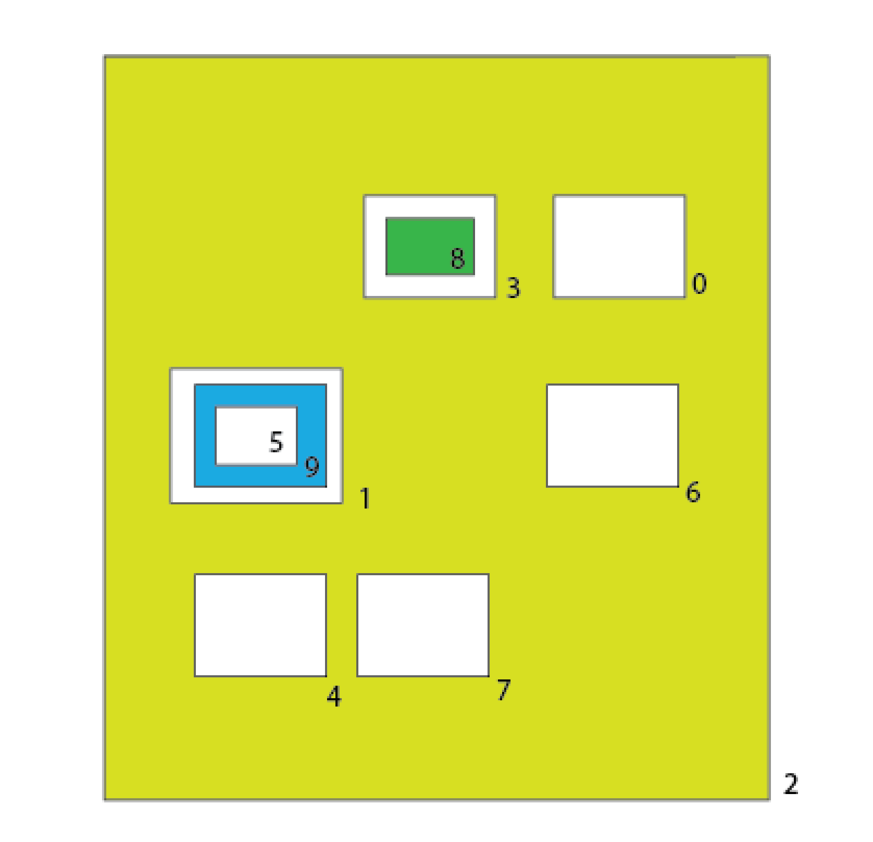
\includegraphics[height=0.24\linewidth,width=0.24\linewidth]{images/lattice0}}
   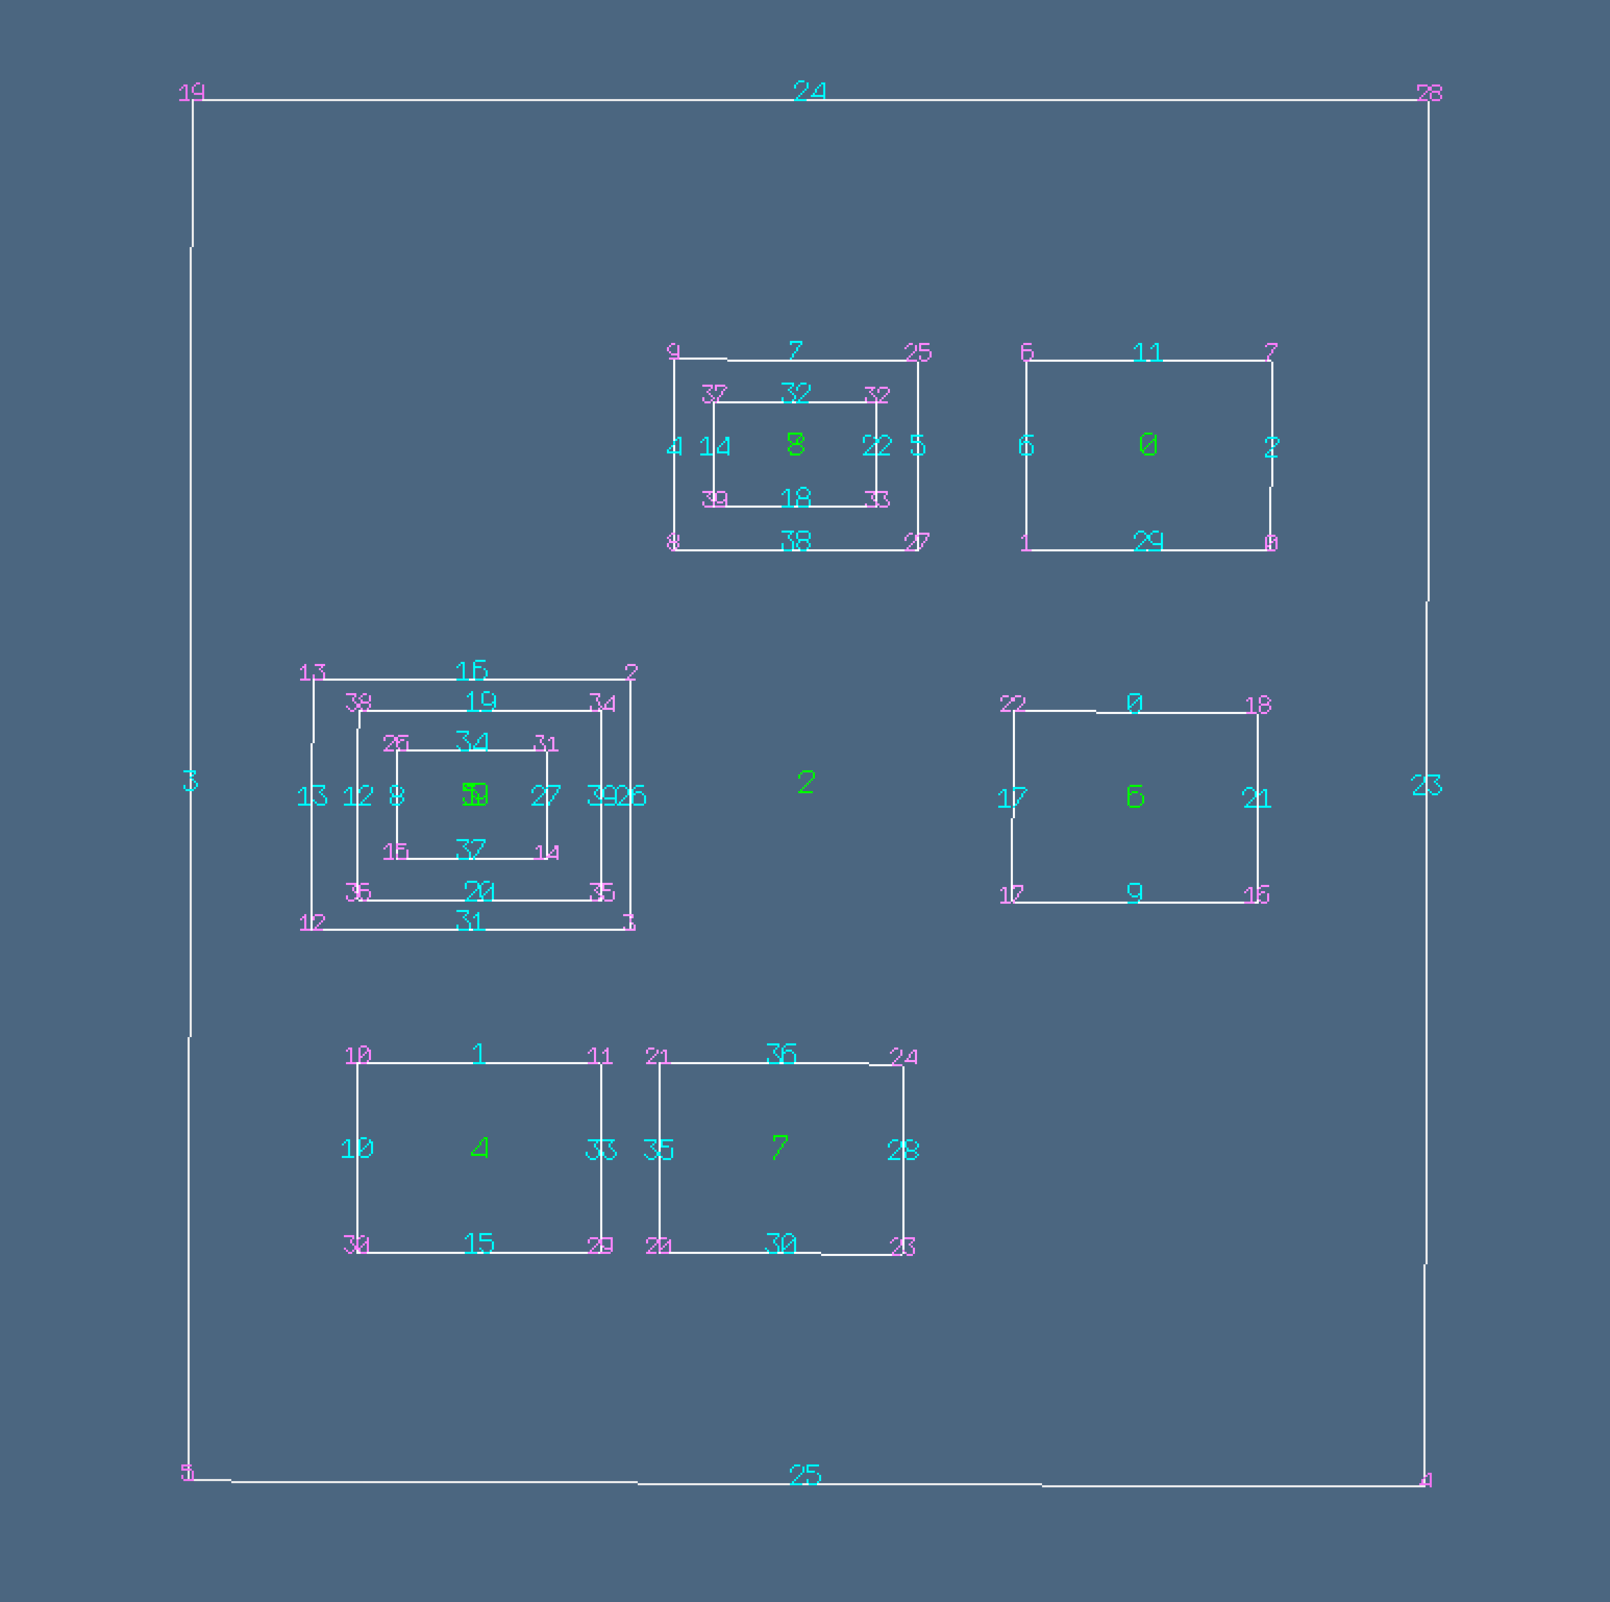
\includegraphics[height=0.24\linewidth,width=0.24\linewidth]{images/lattice1} 
   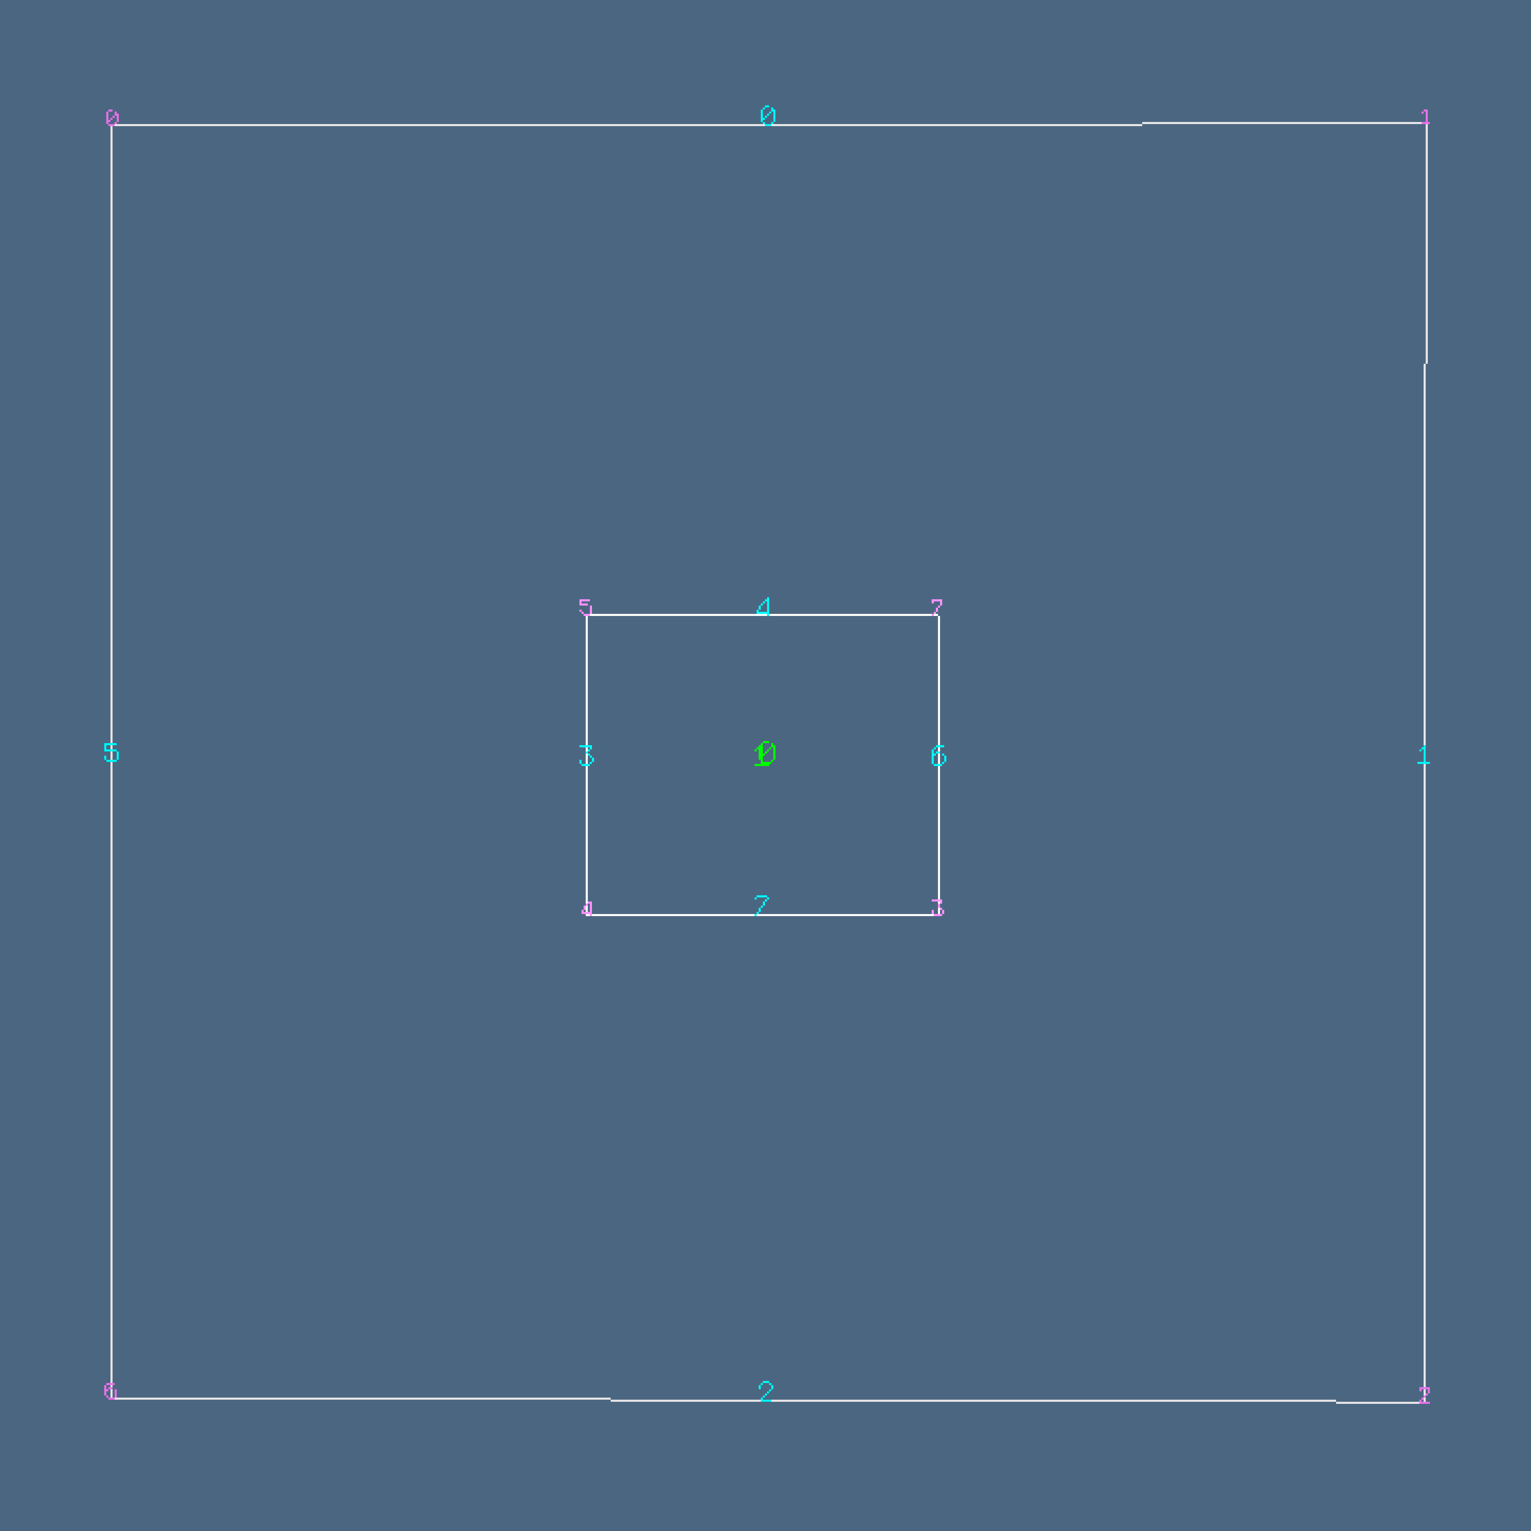
\includegraphics[height=0.24\linewidth,width=0.24\linewidth]{images/lattice2} 
   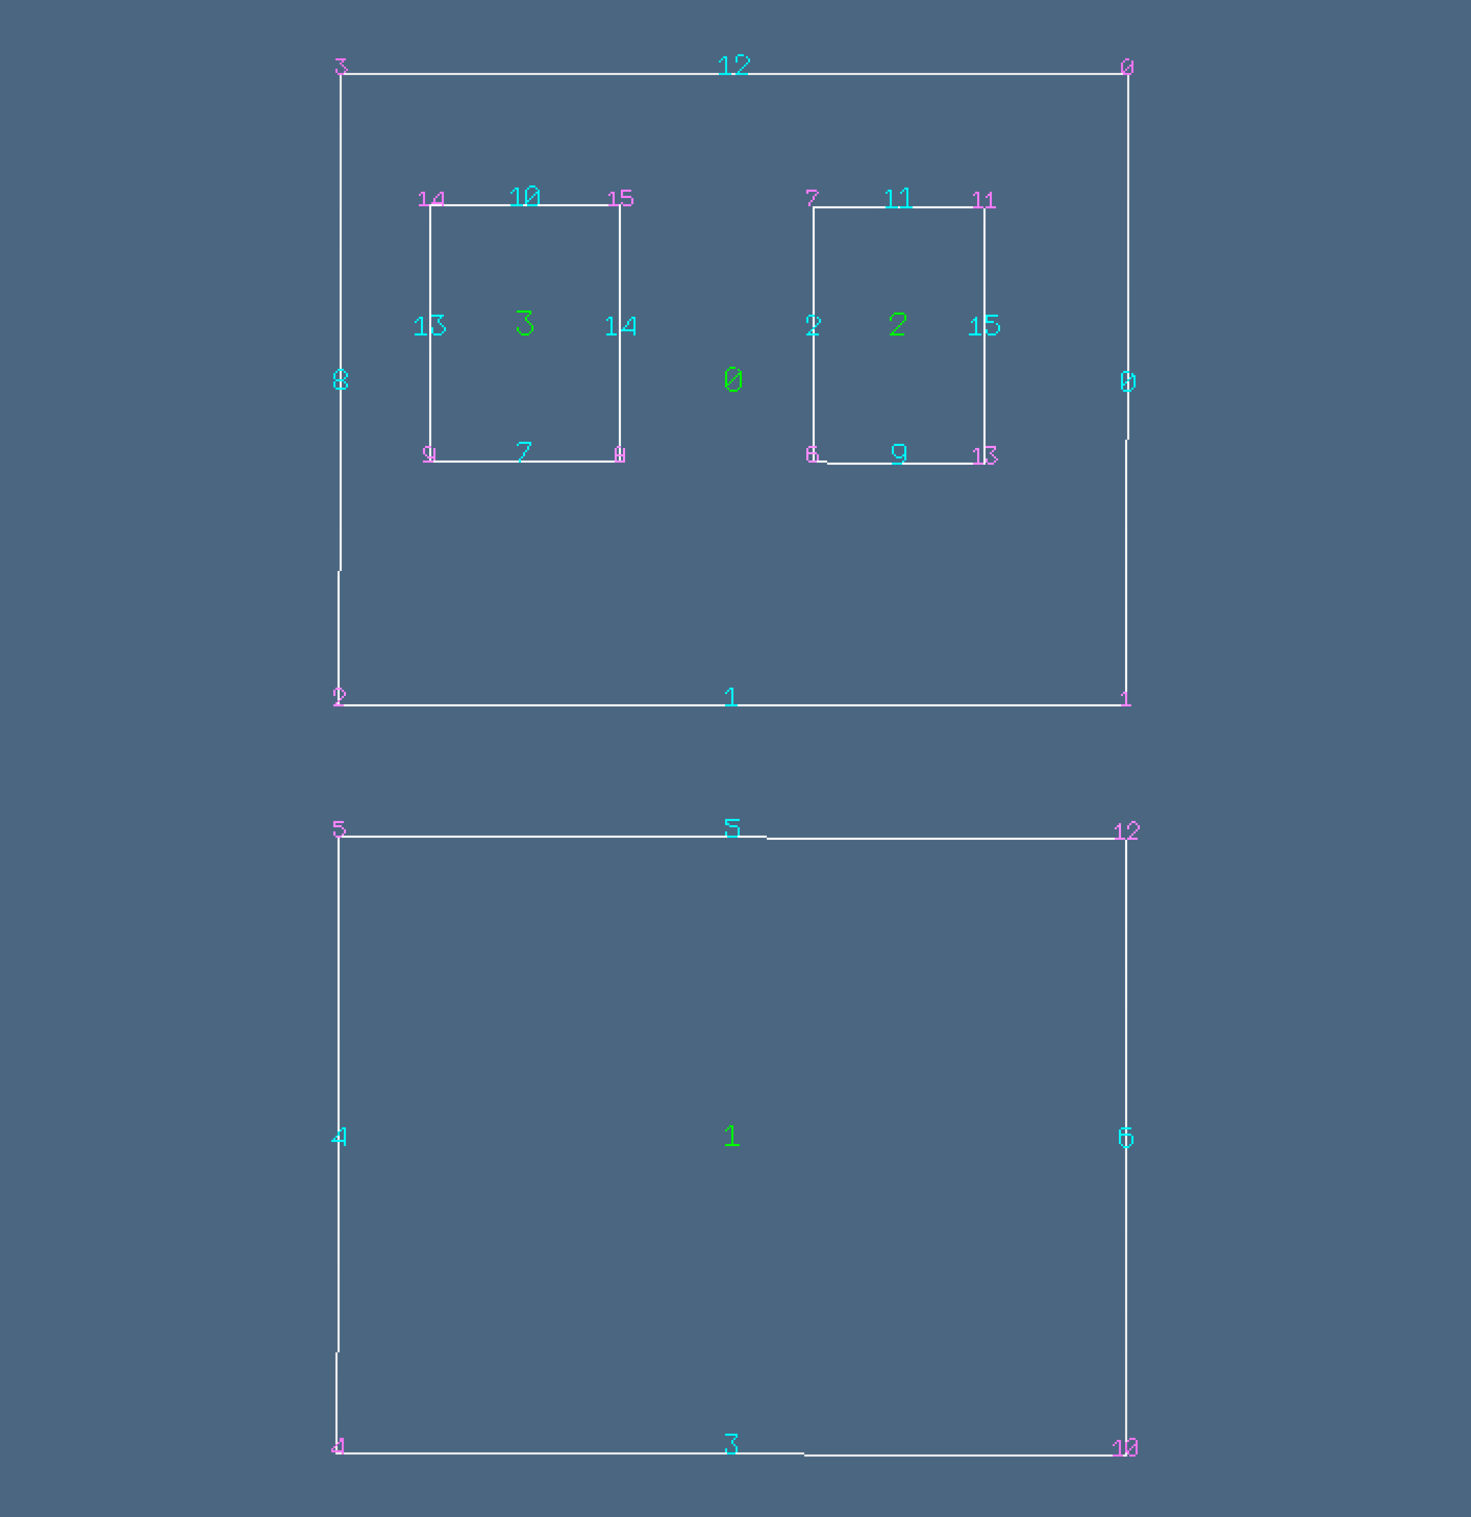
\includegraphics[height=0.24\linewidth,width=0.24\linewidth]{images/lattice3} 
   \caption{Some examples of nested non intersecting cycles. The corresponding solutions are given in the text.}
   \label{fig:example}
\end{figure}


\subsection{Reduction of multiple cycles to a single polyline}
\label{sec:singlepolyline}
%~~~~~~~~~~~~~~~~~~~~~~~~~~~~~~~~~~~~~~~~~~~~~~~~~~~~~~~~~~~~~~~~~~~~~~~~~~~~~~~

The reduction of a lattice of non-intersecting 1-cycles on the boundary of a 2-cell into a single polyline is performed using a scan-line algorithm.

In order to filter the complications induced by edges aligned with the reference axes, first we perform a transformation of vertices from Cartesian to polar coordinates (see Figure~\ref{fig:polarholes}).

Then a specialized scan-line algorithm is executed, producing a set of \emph{bridge-edges}~\cite{Yamaguchi:85} that, added in double instance to the set \texttt{EV} of the LAR of the 2-cell, allow for a triangulation of its interior using the algorithm provided by the \texttt{poly2tria} module.

\begin{figure}[htbp] %  figure placement: here, top, bottom, or page
   \centering
   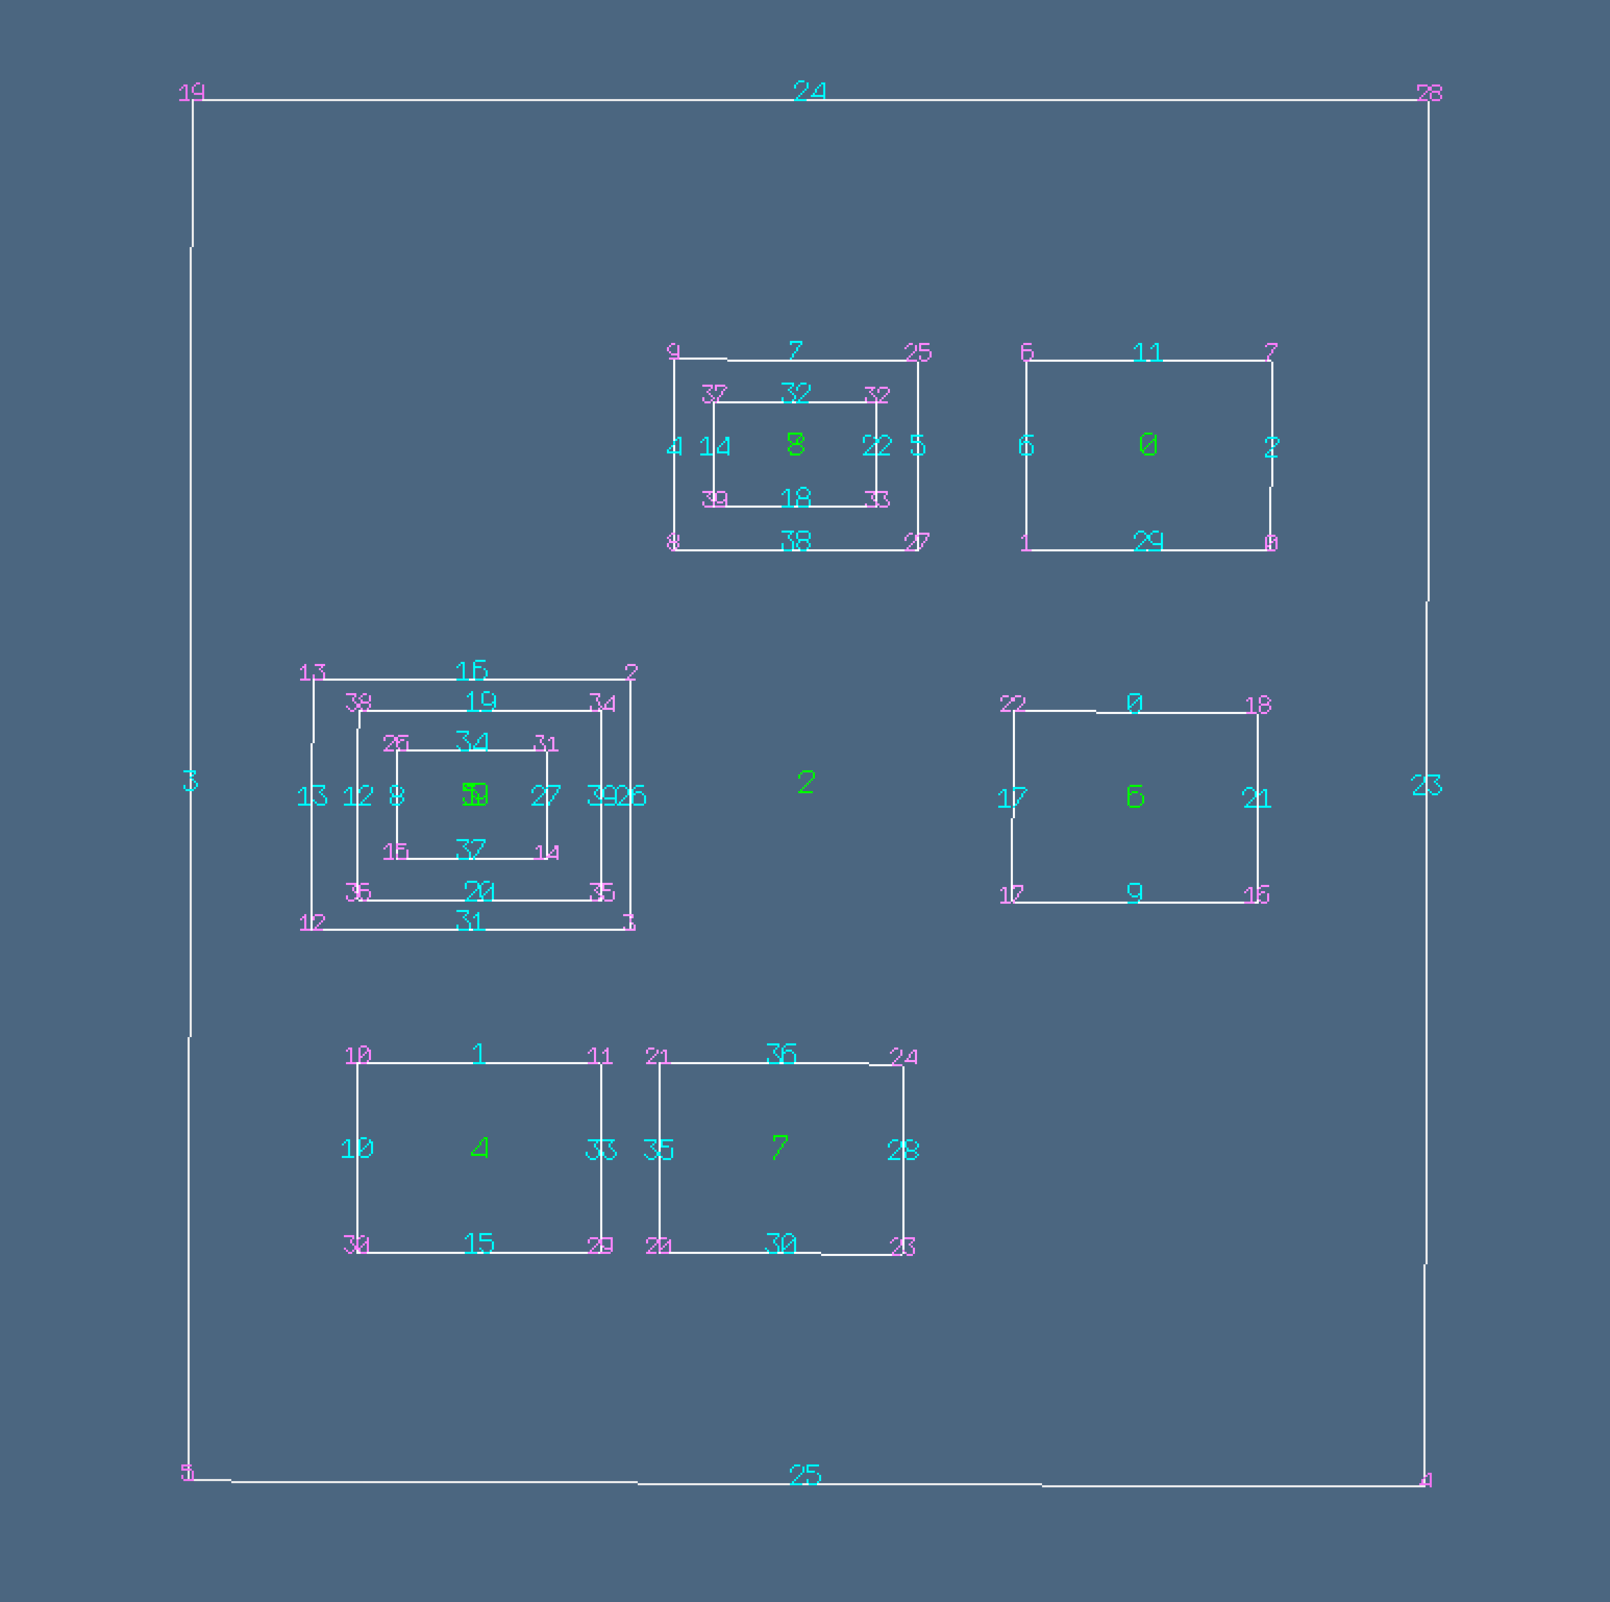
\includegraphics[height=0.33\linewidth,width=0.33\linewidth]{images/lattice1} 
   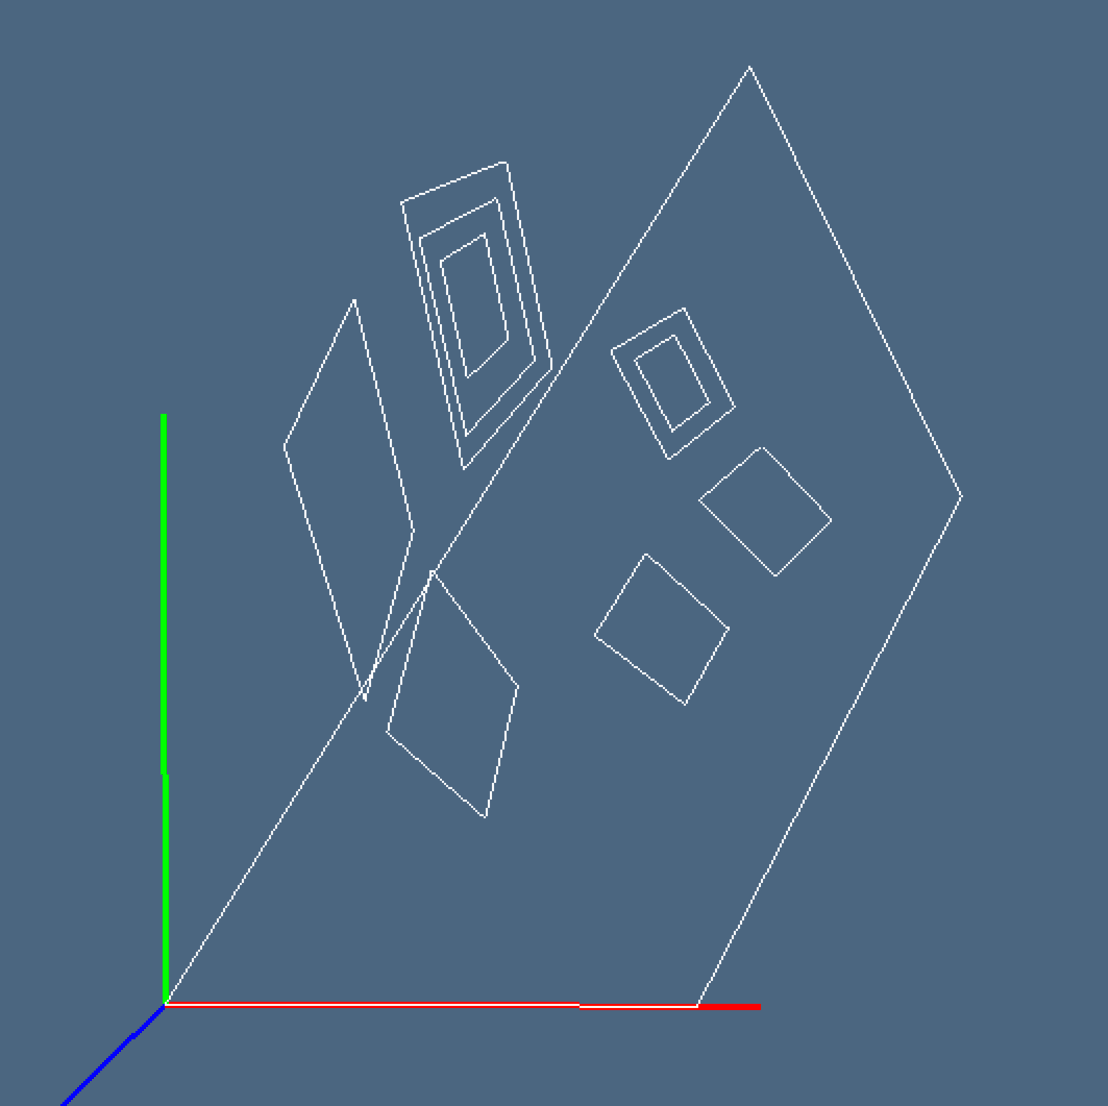
\includegraphics[height=0.33\linewidth,width=0.33\linewidth]{images/polarholes} 
   \caption{A set of non-intersecting boundary cycles in Cartesian and polar coordinates, using (improperly) an Euclidean metric in the transformed space.}
   \label{fig:polarholes}
\end{figure}


\paragraph{Transforming to polar coordinates}

The transformation from Cartesian to polar coordinates of the vertices of a two-dimensional LAR model is given in the following script. An image of such transformation is shown in Figure~\ref{fig:polarholes}. It is only used here to put the vertex coordinates in general position, so simplifying the scan-line algorithm.
%-------------------------------------------------------------------------------
@D Transforming to polar coordinates 
@{""" Transforming to polar coordinates """
def cartesian2polar(V):    
    Z = [[sqrt(x*x + y*y),math.atan2(y,x)] for x,y in V]
    VIEW(STRUCT(MKPOLS((Z,EV))))
    return Z
@}
%-------------------------------------------------------------------------------


\paragraph{Scan line algorithm}
%-------------------------------------------------------------------------------
@D Scan line algorithm 
@{""" Scan line algorithm """
def scan(V,FVs, group,cycleGroup,cycleVerts):
    bridgeEdges = []
    scannedCycles = []
    for k,(point,cycle,v) in enumerate(cycleGroup[:-2]):
    	
        nextCycle = cycleGroup[k+1][1]
        n = len(FVs[group][cycle])
        if nextCycle != cycle: 
            if not ((nextCycle in scannedCycles) and (cycle in scannedCycles)):
                print "k =",k
                scannedCycles += [nextCycle]
                m = len(FVs[group][nextCycle])
                v1,v2 = v,cycleGroup[k+1][2]
                minDist = VECTNORM(VECTDIFF([V[v1],V[v2]]))
                for i in FVs[group][cycle]:
                    for j in FVs[group][nextCycle]:
                        dist = VECTNORM(VECTDIFF([V[i],V[j]]))
                        if  dist < minDist: 
                            minDist = dist
                            v1,v2 = i,j
                bridgeEdges += [(v1,v2)]
    return bridgeEdges[:-1]
@}
%-------------------------------------------------------------------------------

\paragraph{Scan line algorithm input/output}

The two-dimensional LAR \texttt{model} $\equiv$ \texttt{V,EV} was previously created by a \texttt{lines2lar(lines)} expression.

%-------------------------------------------------------------------------------
@D Scan line algorithm input/output
@{""" Scan line algorithm input/output """
def connectTheDots(model):
    V,EV = model
    V,EVs = biconnectedComponent((V,EV))
    FV = AA(COMP([sorted,set,CAT]))(EVs)
    testArray = latticeArray(V,EVs)
    cells = cellsFromCycles(testArray)
    FVs = [[FV[cycle] for cycle in cell] for cell in cells]
    
    indexedCycles = [zip(FVs[h],range(len(FVs[h])))   for h,cell in enumerate(cells)]
    indexedVerts = [CAT(AA(DISTR)(cell)) for cell in indexedCycles]
    sortedVerts = [sorted([(V[v],c,v) for v,c in cell]) for cell in indexedVerts]
    
    bridgeEdges = []
    cellIndices = range(len(cells))
    for (group,cycleGroup,cycleVerts) in zip(cellIndices,sortedVerts,indexedVerts):
        bridgeEdges += [scan(V,FVs, group,cycleGroup,cycleVerts)]
    return cells,bridgeEdges
@}
%-------------------------------------------------------------------------------

\paragraph{Orientation of component cycles of unconnected boundaries}

This step of the algorithm needs some preliminary computation, starting from the list \texttt{EV} of edges by vertices. Just notice that, at this point of the implementation (as the edges of a set of non intersecting cycles) they all are boundary edges, and hence the \texttt{edgeBoundary} variable can be filled with consecutive integers. The \texttt{edgeCycles} returned by \texttt{boundaryCycles} are very well characterized, according to how discussed in the description of the \texttt{Edge cycles associated to a closed chain of edges} paragraph.
The corresponding \texttt{vertexCycles} are first oriented accordingly to \texttt{boundaryCycles}, then rotated (as equivalent permutations) in order to put their element of minimum index in first position (accordingly to the numeration of cycles used in the variable \texttt{FVs}). Then, the \texttt{CVs} will be set to contain the circularly ordered vertices of the various boundary cycles of each LAR 2-cell, in a manner analogous to FVs, where the vertices are not circularly ordered. Finally, the first (i.e.~the \emph{external}) cycle of each cell is counterclockwise oriented, whereas the other cycles (i.e.~the \emph{internal} ones), are oriented clockwise.

%-------------------------------------------------------------------------------
@D Orientation of component cycles of unconnected boundaries 
@{""" Orientation of component cycles of unconnected boundaries """
def rotatePermutation(inputPermutation,transpositionNumber):
    n = transpositionNumber
    perm = inputPermutation
    permutation = range(n,len(perm))+range(n) 
    return [perm[k] for k in permutation]

def canonicalRotation(permutation):
    n = permutation.index(min(permutation))
    return rotatePermutation(permutation,n)

def setCounterClockwise(h,k,cycle,areas,CVs):
    if areas[cycle] < 0.0: 
        chain = copy.copy(CVs[h][k])
        CVs[h][k] = canonicalRotation(REVERSE(chain))

def setClockwise(h,k,cycle,areas,CVs):
    if areas[cycle] > 0.0: 
        chain = copy.copy(CVs[h][k])
        CVs[h][k] = canonicalRotation(REVERSE(chain))

def orientBoundaryCycles(model,cells):
    print "\nmodel =",model
    print "\ncells =",cells
    V,EV = model
    edgeBoundary = range(len(EV))
    edgeCycles,_ = boundaryCycles(edgeBoundary,EV)
    vertexCycles = [[ EV[e][1] if e>0 else EV[-e][0] for e in cycle ] for cycle in edgeCycles]
    print "vertexCycles =",vertexCycles
    rotations = [cycle.index(min(cycle)) for cycle in vertexCycles]
    print "rotations =",rotations
    theCycles = sorted([rotatePermutation(perm,n) for perm,n in zip(vertexCycles,rotations)])
    print "theCycles =",theCycles
    CVs = [[theCycles[cycle] for cycle in cell] for cell in cells]
    print "CVs =",CVs
    areas = signedSurfIntegration((V,theCycles,EV),signed=True)
    print "areas =",areas,"\n"
    
    for h,cell in enumerate(cells):
        for k,cycle in enumerate(cell):
            if k == 0: setCounterClockwise(h,k,cycle,areas,CVs)
            else: setClockwise(h,k,cycle,areas,CVs)
    print "CVs =",CVs
    return CVs
@}
%-------------------------------------------------------------------------------

\paragraph{From nested boundary cycles to triangulation}
%-------------------------------------------------------------------------------
@D From nested boundary cycles to triangulation 
@{""" From nested boundary cycles to triangulation """
def larTriangulation( (V,EV) ):
    model = V,EV
    cells,bridgeEdges = connectTheDots(model)
    CVs = orientBoundaryCycles(model,cells)
    
    polygons = [[[V[u] for u in cycle] for cycle in cell] for cell in CVs]
    triangleSet = []   
    
    for polygon in polygons:
        triangledPolygon = []
        externalCycle = polygon[0]
        polyline = []
        for p in externalCycle:
            polyline.append(Point(p[0],p[1]))
        cdt = CDT(polyline)
        
        internalCycles = polygon[1:]
        for cycle in internalCycles:
            hole = []
            for p in cycle:
                hole.append(Point(p[0],p[1]))
            cdt.add_hole(hole)
            
        triangles = cdt.triangulate()
        trias = [ [[t.a.x,t.a.y,0],[t.c.x,t.c.y,0],[t.b.x,t.b.y,0]] for t in triangles ]
        triangleSet += [AA(REVERSE)(trias)]
    return triangleSet
@}
%-------------------------------------------------------------------------------


\subsection{Monocyclic polygons using bridge-edges}
%~~~~~~~~~~~~~~~~~~~~~~~~~~~~~~~~~~~~~~~~~~~~~~~~~~~~~~~~~~~~~~~~~~~~~~~~~~~~~~~

This subsection, even if correct, is not currently used, since the used triangulation algorithm, from the \texttt{poly2tri} package, cannot handle repeated vertices.

\paragraph{Generation of 1-boundaries as vertex permutation}
In algebraic topology a $k$-cycle is a $k$-chain whose boundary is empty. Also, an unconnected $k$-cycle is the direct sum of two or more $k$-cycles. A good formal representation of every simplicial $k$-cycle, where \emph{each} component $k$-simplex has $k+1$ $(k-1)$-adjacent $k$-simplices is a $(k+1)$-array, indexed by $k$-simplices, i.e.~the \emph{Winged Representation}~\cite{Paoluzzi:1993:DMS:169728.169719}. 

In the case of oriented $1$-cycles, a good representation is given by considering the (ordering of) 0-faces (vertices) as a permutation of $n$ integers, i.e.~as a bijective function $\pi :[0,n]\to[0,n]$ that can be represented as an array \texttt{verts} of integers indexed on integers, and the 1-faces (edges) as a dictionary (mapping) \texttt{nextVert} $verts\to verts$.

In order to join two component cycles using one of \texttt{bridgeEdges}, say $(u,v)$, computed by the function \texttt{connectTheDots} previously given, we must save $\pi(u)$ and $\pi(v)$, say, within $x$ and $y$, respectively
%-------------------------------------------------------------------------------
@D Generation of 1-boundaries as vertex permutation 
@{""" Generation of 1-boundaries as vertex permutation """
def boundaryCycles2vertexPermutation( model ):
    V,EV = model
    cells,bridgeEdges = connectTheDots(model)
    CVs = orientBoundaryCycles(model,cells)
    
    verts = CAT(CAT( CVs ))
    n = len(verts)
    W = copy.copy(V)
    assert len(verts) == sorted(verts)[n-1]-sorted(verts)[0]+1
    nextVert = dict([(v,cycle[(k+1)%(len(cycle))]) for cell in CVs for cycle in cell 
                   for k,v in enumerate(cycle)])
    for k,(u,v) in enumerate(CAT(bridgeEdges)):
        x,y = nextVert[u],nextVert[v]
        nextVert[u] = n+2*k+1
        nextVert[v] = n+2*k      
        nextVert[n+2*k] = x
        nextVert[n+2*k+1] = y
        W += [W[u]]
        W += [W[v]]
        EW = nextVert.items()
    return W,EW
@}
%-------------------------------------------------------------------------------

\paragraph{Wire-frame LAR to boundary polygons}
The 2-dimensional LAR model \texttt{(W,EW)} returned by the function \texttt{boundaryCycles2vertexPermutation} is pretty special, since it is at the same time both a standard LAR model, i.e.~a pair (vertices, edges\_by\_vertices), and a permutation of vertex indices providing implicitly the ordered cycles on the boundary of a 2-complex. In other words, \texttt{EW} is both a (possibly unconnected) 1-cycle and an 1-boundary.

In the following script we extract the list of connected boundaries (including bridge-edges) from the \texttt{EW} permutation of the first $m$ integers.

%-------------------------------------------------------------------------------
@D Wire-frame LAR to boundary polygons 
@{""" lar2boundaryPolygons """
def lar2boundaryPolygons(model):
    W,EW = boundaryCycles2vertexPermutation( model )
    EW = AA(list)(EW)
    polygons = []
    for k,edge in enumerate(EW):
        polygon = []
        if edge[0]>=0:
            first = edge[0]
            done = False
        while (not done) and edge[0] >= 0:
            polygon += [edge[0]]
            edge[0] = -edge[0]
            edge = EW[edge[1]]
            if len(polygon)>1 and polygon[-1] == first: 
                EW[first][0] = -float(first)
                break 
        if polygon != []: 
            if polygon[0]==polygon[-1]: polygon=polygon[:-1]
            polygons += [polygon]
    return W,polygons
@}       
%-------------------------------------------------------------------------------

\begin{figure}[htbp] %  figure placement: here, top, bottom, or page
   \centering
   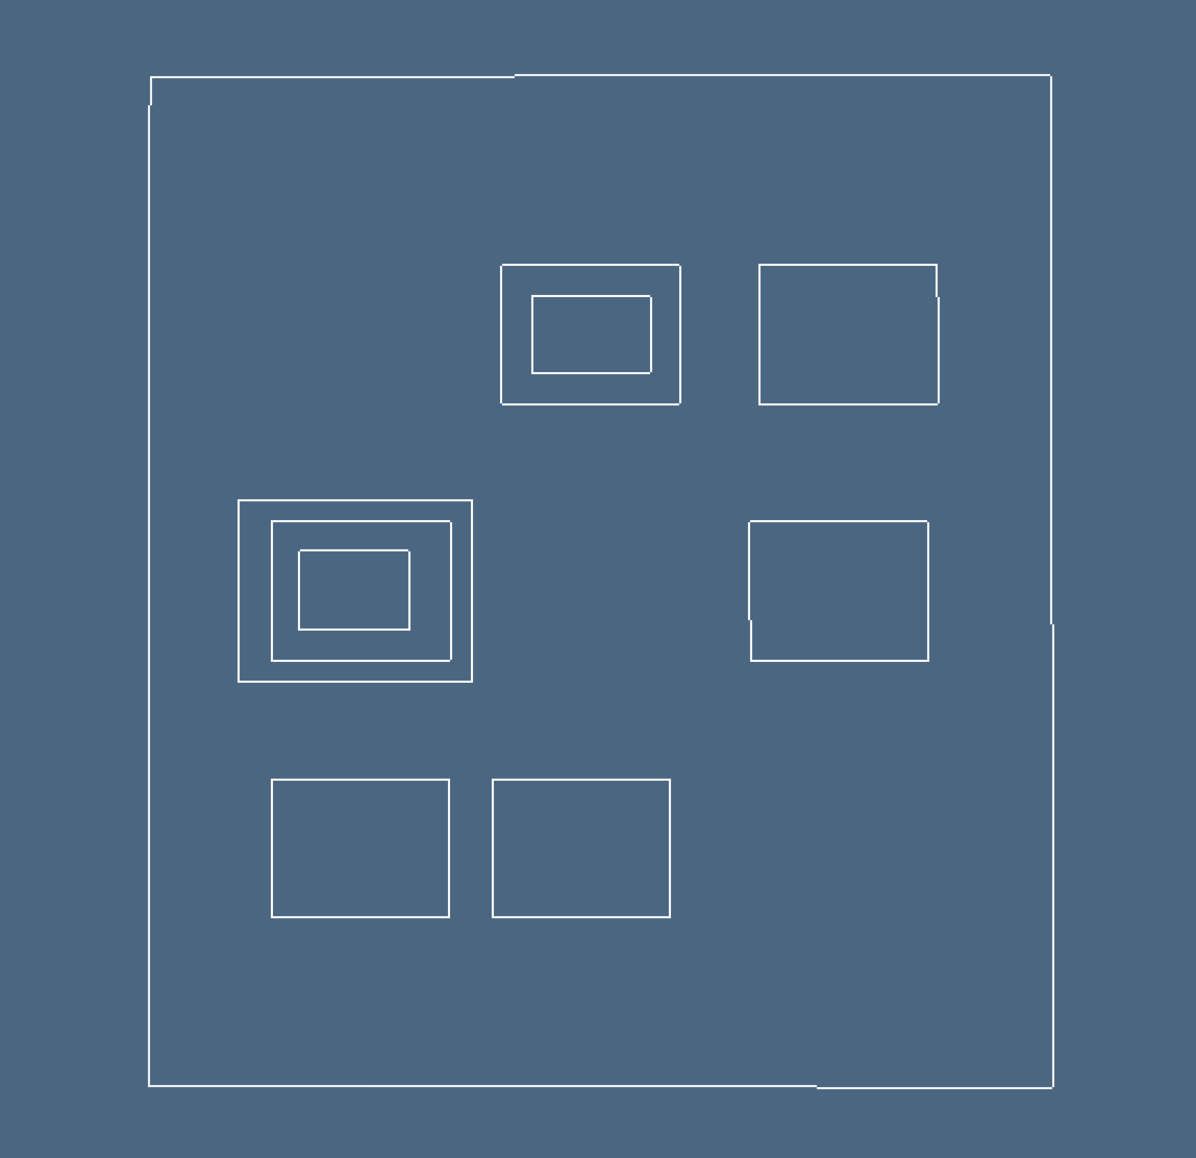
\includegraphics[height=0.32\linewidth,width=0.32\linewidth]{images/holes1}
   
\includegraphics[height=0.32\linewidth,width=0.32\linewidth]{images/holes3} 
   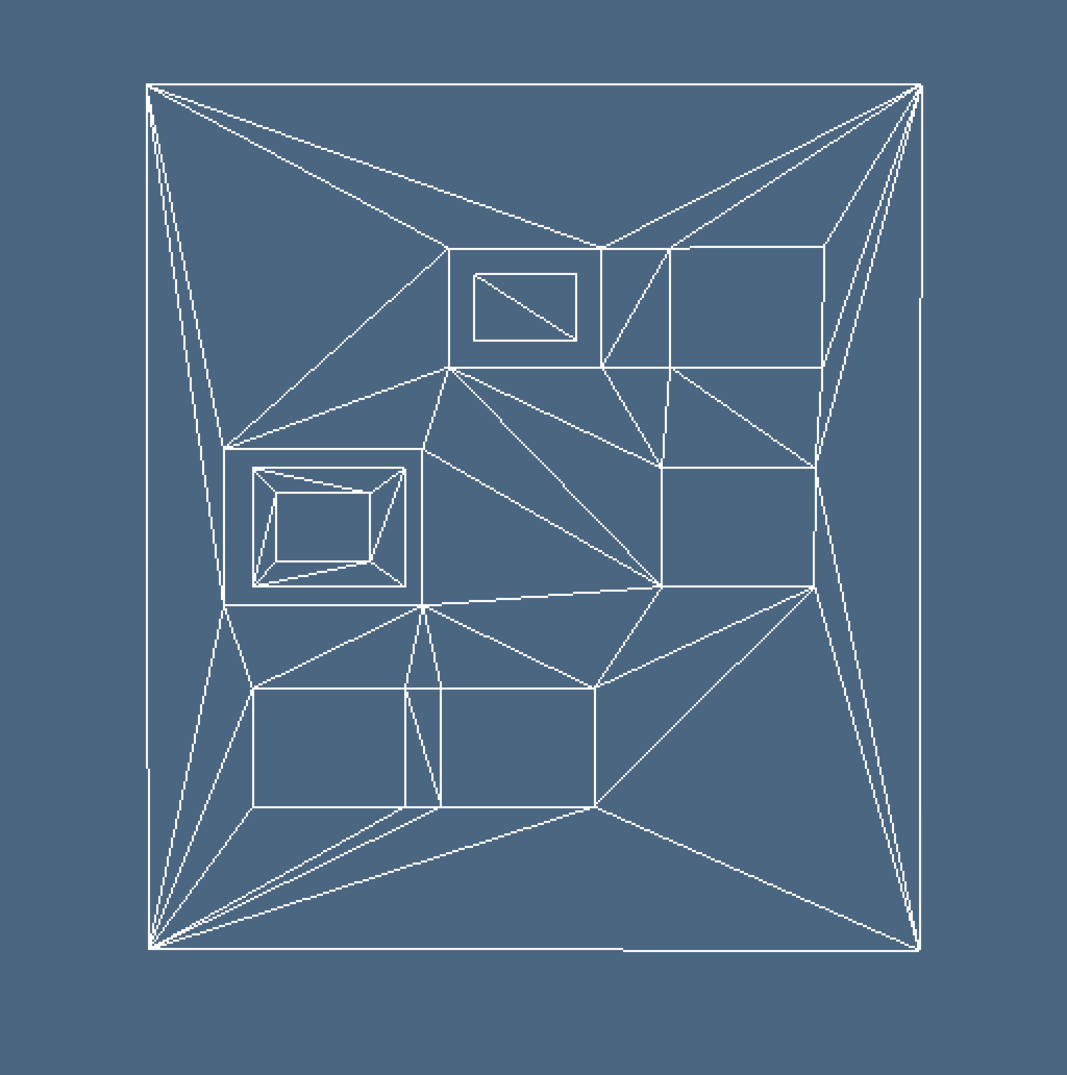
\includegraphics[height=0.32\linewidth,width=0.32\linewidth]{images/holes2} 
   \caption{(a) Closed 1-chain $c$, i.e.~such that $\partial\, c = 0$; $c$ is both cycle and boundary at the same time; (b) 2-chain $h$ such that $\partial\,h = c$; (c) 1-skeleton of a triangulation of $h$.}
   \label{fig:cycles}
\end{figure}


\paragraph{Edge cycles associated to a closed chain of edges}

The output \texttt{cycles} are returned as lists of oriented edges, given in consecutive  sequence in each list. Each cycle is given in the opposite ordering of its first edge.
The first edge of each cycle is the one of minimum index in the cycle. The list of output cycles is returned ordered for increasing (or better, in decreasing order, since negative) order of its first element. The first output cycle starts from index 0, that cannot oriented directly, since -0 is not allowed for integer indices. It must be considered as negative, i.e. as oriented as the opposite of its canonical orientation. 

%-------------------------------------------------------------------------------
@D Edge cycles associated to a closed chain of edges
@{""" Edge cycles associated to a closed chain of edges """

from collections import defaultdict

def detachManifolds(polygonVerts):
    vertCycles = []
    for vertexList in polygonVerts:
        vertCount,counts = defaultdict(list),list
        for v in vertexList: 
            vertCount[v] += [1]
        counts = [sum(vertCount[v]) for v in vertexList]
        vertCycles += [counts]
    return vertCycles
    
def splitManifolds(cycles,vertices,manifolds):
    out = []
    for cycle,verts,manifold in zip(cycles,vertices,manifolds):
        if sum(manifold) == len(manifold):
            out += [cycle] 
        else:
            transpositionNumbers = [n for n,k in enumerate(manifold) if k>1]
            n = transpositionNumbers[0]
            cycle = rotatePermutation(cycle,n) 
            verts = rotatePermutation(verts,n) 
            manifold = rotatePermutation(manifold,n) 
            starts = AA(C(sum)(-n))(transpositionNumbers)+[len(manifold)]
            pairs = [(start,starts[k+1]) for k,start in enumerate(starts[:-1])]
            splitCycles = [[cycle[k] for k in range(*interval)] for interval in pairs]
            splitVerts = [[verts[k] for k in range(*interval)] for interval in pairs]
            out += splitCycles
    return out

def boundaryCycles(edgeBoundary,EV):
    cycles,cycle = [],[]
    vertices = []
    
    def singleBoundaryCycle(edgeBoundary):
        verts2edges = defaultdict(list)
        for e in edgeBoundary:
            verts2edges[EV[e][0]] += [e]
            verts2edges[EV[e][1]] += [e]
        cycle,verts = [],[]
        
        if edgeBoundary == []: return cycle,verts
        e = edgeBoundary[0]
        v,w = EV[e]
        verts = [v,w]
        while edgeBoundary != []:
            cycle += [e]
            edgeBoundary.remove(e)
            v,w = EV[e]
            verts2edges[v].remove(e)
            verts2edges[w].remove(e)
            w = list(set(EV[e]).difference([verts[-1]]))[0]
            if verts2edges[w] == []: break
            e = verts2edges[w][0]
            verts += [w]
        verts = verts[1:]
        return cycle,verts
        
    while edgeBoundary != []:
        edgeBoundary = list(set(edgeBoundary).difference(cycle))
        cycle,verts = singleBoundaryCycle(edgeBoundary)
        if cycle!= []: 
            cycle = [e if verts[k]==EV[e][0] else -e for k,e in enumerate(cycle)]
            cycles += [cycle]
            vertices += [verts]
    manifolds = detachManifolds(vertices)
    cycles = splitManifolds(cycles,vertices,manifolds)
    return cycles,vertices
@}
%-------------------------------------------------------------------------------



\paragraph{From Struct object to LAR boundary model}
%-------------------------------------------------------------------------------
@D From Struct object to LAR boundary model
@{""" From Struct object to LAR boundary model """
def structFilter(obj):
    if isinstance(obj,list):
        if (len(obj) > 1):
            return [structFilter(obj[0])] + structFilter(obj[1:])
        return [structFilter(obj[0])]
    if isinstance(obj,Struct):
        if obj.category in ["external_wall", "internal_wall", "corridor_wall"]:
            return
        return Struct(structFilter(obj.body),obj.name,obj.category)
    return obj

def structBoundaryModel(struct):
    filteredStruct = structFilter(struct)
    #import pdb; pdb.set_trace()
    V,FV,EV = struct2lar(filteredStruct)
    edgeBoundary = boundaryCells(FV,EV)
    cycles,_ = boundaryCycles(edgeBoundary,EV)
    edges = [signedEdge for cycle in cycles for signedEdge in cycle]
    orientedBoundary = [ AA(SIGN)(edges), AA(ABS)(edges)]
    cells = [EV[e] if sign==1 else REVERSE(EV[e]) for (sign,e) in zip(*orientedBoundary)]
    if cells[0][0]==cells[1][0]: # bug badly patched! ... TODO better
        temp0 = cells[0][0]
        temp1 = cells[0][1]
        cells[0] = [temp1, temp0]
    return V,cells
@}
%-------------------------------------------------------------------------------



\paragraph{From structures to boundary polylines}
Notice that the \texttt{if} predicate \texttt{len(V) < len(boundaryEdges)} 
is used to discriminate between manifold (\texttt{False}) and non-manifold (\texttt{True})
boundary cases.
%-------------------------------------------------------------------------------
@D From structures to boundary polylines
@{""" From structures to boundary polylines """
def boundaryPolylines(struct):
    V,boundaryEdges = structBoundaryModel(struct)
    print "\nV =",V
    print "\nboundaryEdges =",boundaryEdges
    if len(V) < len(boundaryEdges):
        EV = AA(sorted)(boundaryEdges)
        boundaryEdges = range(len(boundaryEdges))
        cycles,vertices = boundaryCycles(boundaryEdges,EV)
        print "\ncycles =",cycles
        print "\nvertices =",vertices
        polylines = [[V[v] for v in verts]+[V[verts[0]]] for verts in REVERSE(vertices)]
        print "\npolylines =",polylines,"\n"
    else:
        polylines = boundaryModel2polylines((V,boundaryEdges))
    print "\npolylines =",polylines,"\n"
    return polylines
@}
%-------------------------------------------------------------------------------


\paragraph{From LAR oriented boundary model to polylines}
%-------------------------------------------------------------------------------
@D From LAR boundary model to polylines
@{""" From LAR oriented boundary model to polylines """
def boundaryModel2polylines(model):
    if len(model)==2: V,EV = model
    elif len(model)==3: V,FV,EV = model
    polylines = []
    succDict = dict(EV)
    visited = [False for k in range(len(V))]
    nonVisited = [k for k in succDict.keys() if not visited[k]]
    while nonVisited != []:
        first = nonVisited[0]; v = first; polyline = []
        while visited[v] == False:
            visited[v] = True; 
            polyline += V[v], 
            v = succDict[v]
        polyline += [V[first]]
        polylines += [polyline]
        nonVisited = [k for k in succDict.keys() if not visited[k]]
    return polylines

def boundaryModel2polylines(model):
    if len(model)==2: V,EV = model
    elif len(model)==3: V,FV,EV = model
    polylines = []
    succDict = dict(EV)
    visited = [False for k in range(len(V))]
    nonVisited = [k for k in succDict.keys() if not visited[k]]
    while nonVisited != []:
        first = nonVisited[0]; v = first; polyline = []
        while visited[v] == False:
            visited[v] = True; 
            polyline += V[v], 
            v = succDict[v]
        polyline += [V[first]]
        polylines += [polyline]
        nonVisited = [k for k in succDict.keys() if not visited[k]]
    return polylines
@}
%-------------------------------------------------------------------------------





\subsection{Visualization of a 2D complex and 2-chain}

%-------------------------------------------------------------------------------
@D Visualization of a 2D complex and 2-chain
@{""" Visualization of a 2D complex and 2-chain """
def larComplexChain(model):
    V,FV,EV = model
    VV = AA(LIST)(range(len(V)))
    csrBoundaryMat = boundary1(FV,EV,VV)
    def larComplexChain0(chain):
        boundaryChain = chain2BoundaryChain(csrBoundaryMat)(chain)
        outModel = V,[EV[e] for e in boundaryChain]
        triangleSet = larTriangulation(outModel)
        return boundaryChain,triangleSet
    return larComplexChain0
    
def viewLarComplexChain(model):
    V,FV,EV = model
    operator = larComplexChain(model)
    def viewLarComplexChain0(chain):
        boundaryChain,triangleSet = operator(chain)
        hpcChain = AA(JOIN)(AA(AA(MK))(CAT(triangleSet)))
        hpcChainBoundary = AA(COLOR(RED))(MKPOLS((V,[EV[e] for e in boundaryChain])))
        VIEW(STRUCT( hpcChain + hpcChainBoundary ))
        VIEW(EXPLODE(1.2,1.2,1.2)( hpcChain + hpcChainBoundary ))
    return viewLarComplexChain0
@}
%-------------------------------------------------------------------------------




\subsection{Point in polygon classification}


%-------------------------------------------------------------------------------
@D Point in polygon testing
@{""" Point-in-polygon classification algorithm """
@< Half-line crossing test @>
@< Tile codes computation @>
@< Point-in-polygon classification algorithm @>
@}
%-------------------------------------------------------------------------------

\paragraph{Tile codes computation}
%-------------------------------------------------------------------------------
@D Tile codes computation
@{""" Tile codes computation """
def setTile(box):
    tiles = [[9,1,5],[8,0,4],[10,2,6]]
    b1,b2,b3,b4 = box
    def tileCode(point):
        x,y = point
        code = 0
        if y>b1: code=code|1
        if y<b2: code=code|2
        if x>b3: code=code|4
        if x<b4: code=code|8
        return code 
    return tileCode
@}
%-------------------------------------------------------------------------------


\paragraph{Half-line crossing test}
%-------------------------------------------------------------------------------
@D Half-line crossing test 
@{""" Half-line crossing test """
def crossingTest(new,old,count,status):
    if status == 0:
        status = new
        count += 0.5
    else:
        if status == old: count += 0.5
        else: count -= 0.5
        status = 0
@}
%-------------------------------------------------------------------------------

\paragraph{Point in polygon testing}
%-------------------------------------------------------------------------------
@D Point-in-polygon classification algorithm
@{""" Point in polygon classification """
def pointInPolygonClassification(pol):

    V,EV = pol
    # edge orientation
    FV = [sorted(set(CAT(EV)))]
    orientedCycles = boundaryPolylines(Struct([(V,FV,EV)]))
    EV = []
    for cycle in orientedCycles:
        EV += zip(cycle[:-1],cycle[1:])

    def pointInPolygonClassification0(p):
        x,y = p
        xmin,xmax,ymin,ymax = x,x,y,y
        tilecode = setTile([ymax,ymin,xmax,xmin])
        count,status = 0,0
    
        for k,edge in enumerate(EV):
            p1,p2 = edge[0],edge[1]
            (x1,y1),(x2,y2) = p1,p2
            c1,c2 = tilecode(p1),tilecode(p2)
            c_edge, c_un, c_int = c1^c2, c1|c2, c1&c2
            
            if c_edge == 0 and c_un == 0: return "p_on"
            elif c_edge == 12 and c_un == c_edge: return "p_on"
            elif c_edge == 3:
                if c_int == 0: return "p_on"
                elif c_int == 4: count += 1
            elif c_edge == 15:
                x_int = ((y-y2)*(x1-x2)/(y1-y2))+x2 
                if x_int > x: count += 1
                elif x_int == x: return "p_on"
            elif c_edge == 13 and ((c1==4) or (c2==4)):
                    crossingTest(1,2,status,count)
            elif c_edge == 14 and (c1==4) or (c2==4):
                    crossingTest(2,1,status,count)
            elif c_edge == 7: count += 1
            elif c_edge == 11: count = count
            elif c_edge == 1:
                if c_int == 0: return "p_on"
                elif c_int == 4: crossingTest(1,2,status,count)
            elif c_edge == 2:
                if c_int == 0: return "p_on"
                elif c_int == 4: crossingTest(2,1,status,count)
            elif c_edge == 4 and c_un == c_edge: return "p_on"
            elif c_edge == 8 and c_un == c_edge: return "p_on"
            elif c_edge == 5:
                if (c1==0) or (c2==0): return "p_on"
                else: crossingTest(1,2,status,count)
            elif c_edge == 6:
                if (c1==0) or (c2==0): return "p_on"
                else: crossingTest(2,1,status,count)
            elif c_edge == 9 and ((c1==0) or (c2==0)): return "p_on"
            elif c_edge == 10 and ((c1==0) or (c2==0)): return "p_on"
        if ((round(count)%2)==1): return "p_in"
        else: return "p_out"
    return pointInPolygonClassification0
@}
%-------------------------------------------------------------------------------


\section{Exporting the library}
%===============================================================================

%-------------------------------------------------------------------------------
@O larlib/larlib/triangulation.py
@{""" Module for pipelined intersection of geometric objects """
from larlib import *

@< Edge cycles associated to a closed chain of edges @>
@< Point in polygon testing @>
@< Classification of non intersecting cycles @>
@< Extraction of path-connected boundaries @>
@< Transforming to polar coordinates @>
@< Scan line algorithm @>
@< Scan line algorithm input/output @>
@< Orientation of component cycles of unconnected boundaries @>
@< From nested boundary cycles to triangulation @>
@< Generation of 1-boundaries as vertex permutation @>
@< Wire-frame LAR to boundary polygons @>
@< From Struct object to LAR boundary model @>
@< From structures to boundary polylines @>
@< From LAR boundary model to polylines @>
@< Visualization of a 2D complex and 2-chain @>
@}
%-------------------------------------------------------------------------------


\section{Testing}
%===============================================================================

In order to test the algorithms implemented in this library, we make use of random triangulations of $C_2=\{x\in\R^2: \norm{x}\leq 1\}$.

\begin{figure}[htbp] %  figure placement: here, top, bottom, or page
   \centering
   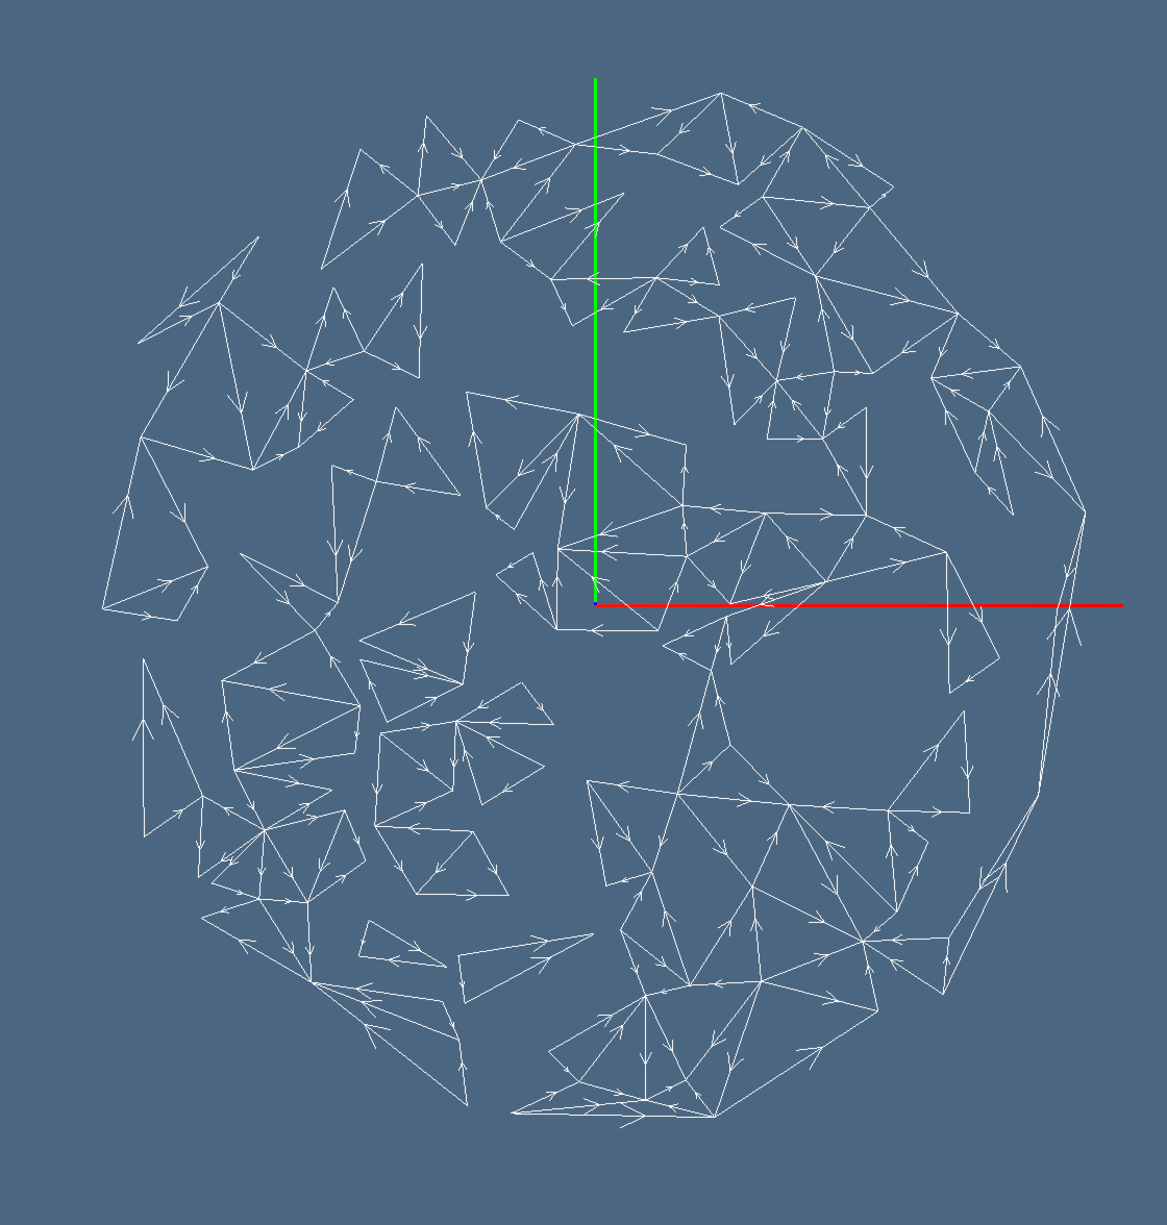
\includegraphics[width=0.33\linewidth]{images/alg-tria0} 
   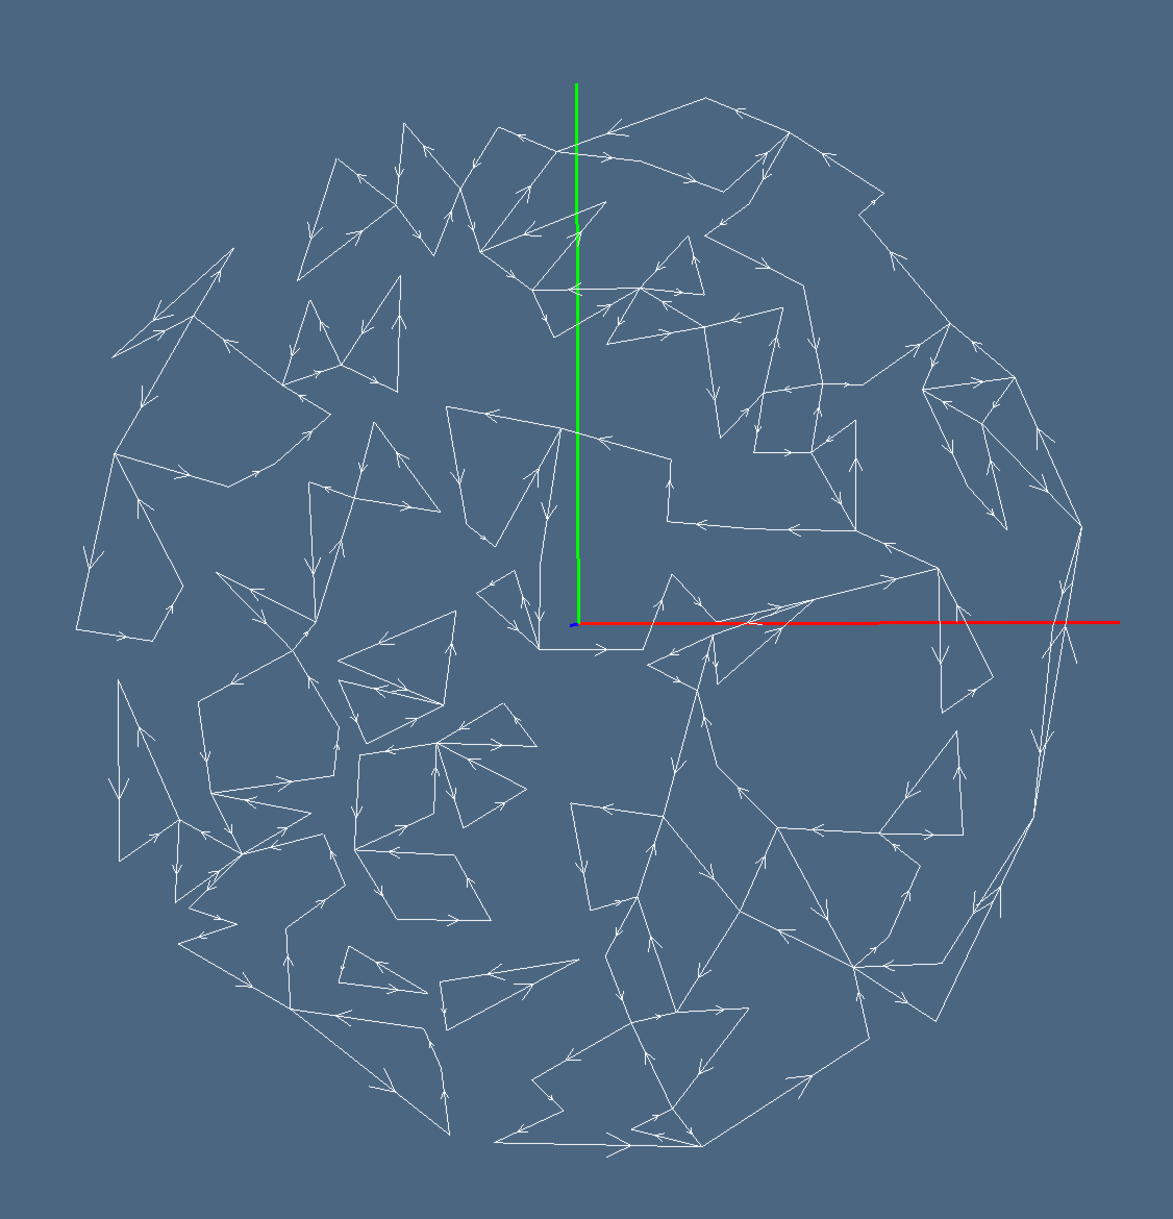
\includegraphics[width=0.33\linewidth]{images/alg-tria1} 
   \caption{example caption}
   \label{fig:example}
\end{figure}

%-------------------------------------------------------------------------------
@O test/py/triangulation/test01.py
@{
from larlib import *

@< random 1-boundary generation @>
@}
%-------------------------------------------------------------------------------

\paragraph{random 1-boundary generation}

%-------------------------------------------------------------------------------
@D random 1-boundary generation
@{""" random 1-boundary generation """
import sys
sys.path.insert(0, '/Users/paoluzzi/Documents/dev/lar-cc/test/py/larcc/')
from test16 import *

EV = AA(list)(cells)
V,EVs = biconnectedComponent((V,EV))
FV = AA(COMP([sorted,list,set,CAT]))(EVs)
FV = sorted( FV,key=len,reverse=True )
EVs = sorted( EVs,key=len,reverse=True )
W = [eval(vcode(v)) for v in V]
testArray = latticeArray(W,EVs)

"""
bcycles,bverts = boundaryCycles(range(len(EW)),EW)
VIEW(STRUCT(AA(POLYLINE)([[V[v] for v in verts] for verts in bverts])))
"""
    
colors = [CYAN, MAGENTA, WHITE, RED, YELLOW, GRAY, GREEN, ORANGE, BLACK, BLUE, 
			PURPLE, BROWN]
components = [COLOR(colors[k%12])(STRUCT(MKPOLS((V,ev)))) for k,ev in enumerate(EVs)]
VIEW(STRUCT(components))
@}
%-------------------------------------------------------------------------------






\bibliographystyle{amsalpha}
\bibliography{triangulation}

\end{document}
